\documentclass[12pt, twoside]{article}
\usepackage[letterpaper, margin=1in, headsep=0.2in]{geometry}
\setlength{\headheight}{0.6in}
%\usepackage[english]{babel}
\usepackage[utf8]{inputenc}
\usepackage{microtype}
\usepackage{amsmath}
\usepackage{amssymb}
%\usepackage{amsfonts}
\usepackage{siunitx} %units in math. eg 20\milli\meter
\usepackage{yhmath} % for arcs, overparenth command
\usepackage{tikz} %graphics
\usetikzlibrary{quotes, angles}
\usepackage{graphicx} %consider setting \graphicspath{{images/}}
\usepackage{parskip} %no paragraph indent
\usepackage{enumitem}
\usepackage{multicol}
\usepackage{venndiagram}

\usepackage{fancyhdr}
\pagestyle{fancy}
\fancyhf{}
\renewcommand{\headrulewidth}{0pt} % disable the underline of the header
\raggedbottom
\hfuzz=2mm %suppresses overfull box warnings

\usepackage{hyperref}

\fancyhead[LE]{\thepage}
\fancyhead[RO]{\thepage \\ Name: \hspace{4cm} \,\\}
\fancyhead[LO]{BECA / Dr. Huson / Geometry\\*  Unit 12: Trigonometry \\* 14 March 2023}

\begin{document}

\subsubsection*{12.2 Homework: Tangent applications \hfill CCSS.HSG.SRT.C.8}
For a right triangle, $\displaystyle \tan \theta = \frac{\rm{opposite}}{\rm{adjacent}}$
\begin{enumerate}
\item Do Now: Given right $\triangle JKL$ with $\overline{JK} \perp \overline{KL}$, $JK=10$, $m\angle J=31^\circ$. Let $x$ be the length of the side opposite $\angle J$, $x=KL$.
\begin{enumerate}
  \item Mark up the triangle.
  \item Find $x$.
\end{enumerate}
    \begin{flushright}
        \begin{tikzpicture}[scale=0.7, rotate=20]
          \draw [thick](0,0)--(6,0)--(6,3)--cycle;
          \draw [fill] (0,0) circle [radius=0.05] node[below]{$J$};
          \draw [fill] (6,0) circle [radius=0.05] node[below]{$K$};
          \draw [fill] (6,3) circle [radius=0.05] node[above right]{$L$};
        \end{tikzpicture}
      \end{flushright}

\item $\triangle ABC$ is shown with $m\angle C=90^\circ$ and the lengths of the triangle's sides are $AC=8$, $BC=15$.  \hfill (not drawn to scale)
  \begin{multicols}{2}
    \begin{enumerate}
      \item Write down the value of $\tan A$. \vspace{1.25cm}
      \item Find the measure of $\angle A$. \vspace{1cm}
      \item Write down the value of $\tan B$. \vspace{1.25cm}
      \item Find the measure of $\angle B$ two different ways. \vspace{1cm}
      \item Find $AB$.
    \end{enumerate}
    \begin{flushright}
    \begin{tikzpicture}[scale=0.5]
      \draw [thick]
      (0,0)node[left]{$A$}--
      (8,0)node[ right]{$C$}--
      (8,15)node[right]{$B$}--cycle;
      \draw (8,0)++(-0.6,0)--++(0,0.6)--+(0.6,0);
      \node at (4,0)[below]{$8$};
      \node at (8,8)[right]{$15$};
      %\node at (2.5,6)[above]{$17$};
    \end{tikzpicture}
    \end{flushright}
  \end{multicols}
  \vspace{3cm}

\newpage
\item Romeo is standing 8 meters away from Juliet's house, looking up at Juliet's window. He is two meters tall and looks up at a $55^\circ$ angle.\\[0.25cm]
Find the height of Juliet's window ledge to the \emph{nearest meter}. \hfill (not drawn to scale)
  \begin{flushright}
    \begin{tikzpicture}[scale=0.3]
      \draw [-, dashed] (0,2)--(3,2);
      \draw [-, thick] (-4,0)--
      (0,0)--
        (10,0)--(10,10)--(12,10);
      \draw [fill] (0,0) circle [radius=0.1] node[above]{Romeo};
      \draw [fill] (10,10) circle [radius=0.1] node[above right]{Window};
      \draw [dashed] (0,2)--(10,10);
      \node at (3, 2)[above]{$55^\circ$};
      \node at (12, 0)[above]{house};
      \node at (12.5, 3)[above]{Juliet's };
    \end{tikzpicture}
    \end{flushright}
    

\item From the top of a lighthouse, a ship is visible at an angle of depression of $3^\circ$. If the lighthouse is 1000 meters tall, determine the distance of the ship from the lighthouse, $x$, to the \emph{nearest kilometer}.
\begin{center}
    \begin{tikzpicture}[scale=1.1]
      \draw [thick] (10,0)--(0,0)--(10,2.0)--cycle;
      \draw [dashed, <-] (5,2)--(10,2.0);
      \draw [thick, ->] (8.5,2) arc [start angle=180, end angle=191.3, radius=1.5];
      \node at (5.5,2)[below]{Angle of depression $=3^\circ$};
      \node at (10,1.2)[right]{height $=1000$ meters};
      \node at (6,0)[below]{$x$};
      \node at (0,0)[below]{Ship};
    \end{tikzpicture}
  \end{center} \vspace{2cm}

\item An airplane flying at an altitude of 3,000 meters is observed twice. The first time the angle of elevation is $5^\circ$ and exactly one minute later the angle of elevation is $7.5^\circ$. \\[0.25cm]
Find the distance the plane flies over the minute and its speed in kilometers per hour.
\begin{flushright}
  \begin{tikzpicture}[scale=1.1]
    \draw [thick] (10,0)--(0,0)--(10,2.0)--cycle;
    \draw [dashed] (0,0)--(7,2.0);
    \draw [dashed, <-] (6,2)--(10,2);
    \draw [thick, ->] (1.5,0) arc [start angle=0, end angle=11.3, radius=1.5];
    \draw [thick, ->] (2.5,0) arc [start angle=0, end angle=15.3, radius=2.5];
    \node at (1,0.7)[above]{Angles of elevation};
    \node at (1.5,0)[below]{$5^\circ$};
    \node at (3,0)[above]{$7.5^\circ$};
    \node at (10,1.2)[left]{$3000$};
    \node at (8,2)[above]{plane};
  \end{tikzpicture} 
\end{flushright}
\vspace{4cm}

\newpage
\item Shown is a building with student $A$ on the ground waving up to student $B$. Point $A$ is 19 feet from the base of the building, and the angle of elevation from $A$ to $B$ is $32^\circ$.
 
Find how high up student B is from the ground to the \emph{nearest foot}. \hfill (not to scale)
  \begin{flushright}
    \begin{tikzpicture}[scale=0.3]
      %\draw [-, thick] (0,0)--(35:23);
      \draw [-, thick] (-4,0)--
      (0,0)--
        (17,0)--
        (22,0)--
        (22,10)--(17,10)--(17,0);
      \draw [fill] (0,0) circle [radius=0.1] node[above left]{$A$};
      \draw [fill] (17,10) circle [radius=0.1] node[above right]{$B$};
      \draw [dashed] (0,0)--(17,10);
      \node at (3.8, 0)[above]{$32^\circ$};
      \node at (11, 0)[above]{distance = 19 ft};
      \node at (19.5, 5)[above]{school};
    \end{tikzpicture}
    \end{flushright}

\item From the top of a subway station, a person is visible at an angle of depression of $21^\circ$. If the subway station is 60 feet tall, determine the distance from the person to the base of the subway station, x, to the \emph{nearest foot}.
\begin{flushright}
    \begin{tikzpicture}[scale=1.1]
      \draw [thick] (10,0)--(0,0)--(10,2.0)--cycle;
      \draw [dashed, <-] (5,2)--(10,2.0);
      \draw [thick, ->] (8.5,2) arc [start angle=180, end angle=191.3, radius=1.5];
      \node at (5.5,2)[below]{Angle of depression $=21^\circ$};
      \node at (10,1)[left]{$h=60$};
      \node at (6,0)[below]{$x$};
      \node at (0,0)[below]{Person};
    \end{tikzpicture}
  \end{flushright} \vspace{1.5cm}

\item A child sleds from the top of a hill to a group of friends standing at the base of the hill. The hill is 21 feet tall, and the hill's incline is $13^\circ$. Find the distance, $d$, from the sledder to the group of friends to the \emph{nearest foot}.

(hint: First find the horizontal distance, the base of the triangle. Then use the Pythagorean theorem to find the hypotenuse, $d$.)
\begin{flushright}
  \begin{tikzpicture}[scale=1.1]
    \draw [thick] (10,0)--(0,0)--(10,2.0)--cycle;
    \draw [thick, ->] (1.5,0) arc [start angle=0, end angle=11.3, radius=1.5];
    \node at (1,0)[below]{Incline $=13^\circ$};
    \node at (10,1.2)[left]{$21$};
    \node at (5,1.6)[below]{$d$};
  \end{tikzpicture} 
\end{flushright}\vspace{4cm}

\newpage
\item A pirate, who is two meters tall, is standing on a mast 8 meters tall. Looking down, the pirate sees an enemy ship 45 meters away.

  Find the angle of depression to the nearest degree.
  \begin{center}
      \begin{tikzpicture}[scale=1.1]
        \draw [thick] (10,0)--(0,0)--(10,2.0)--cycle;
        \draw [dashed, <-] (5,2)--(10,2.0);
        \draw [thick, ->] (8.5,2) arc [start angle=180, end angle=191.3, radius=1.5];
        \node at (5.5,2)[below]{Angle of depression $ =\theta^\circ$};
        \node at (10,1.2)[right]{$h=8+2$ meters};
        \node at (6,0)[below]{$45 \,\rm{meters}$};
        \node at (0,0)[below right]{Enemy ship};
      \end{tikzpicture}
    \end{center} \vspace{4cm}
    
\item A snowman is standing 10 meters away from the base of a set of monkey bars, looking up at a boy 3 meters off the ground. The snowman is 1 meter tall.

    (a) Mark the triangle.
    
    (b) Find the angle from the snowman's head to the boy, $\theta$, to the nearest tenth degree.
    
     \hfill (not drawn to scale)
      \begin{flushright}
        \begin{tikzpicture}[scale=0.6]
          \draw [-, dashed] (0,2)--(3,2);
          \draw [-, thick] (-4,0)--
          (0,0)--
            (10,0)--(10,6)--(12,6);
          \draw (0,0.75) circle [radius=0.75];
          \draw (0,2) circle [radius=0.5];
          \draw [fill] (10,6) circle [radius=0.1] node[above right]{Boy};
          \draw [dashed] (0,2)--(10,6);
          \node at (3, 2)[above]{$ \theta^\circ$};
          \node at (12, 2)[above]{Bars};
          \node at (12.5, 3)[above]{Monkey};
        \end{tikzpicture}
        \end{flushright}

\newpage
\item Given right $\triangle ABC$ with $AC=10$, $m\angle A=40^\circ$. Find the value of $BC=x$.
  \begin{flushright}
    \begin{tikzpicture}[scale=0.6]
      \draw [thick](-1,0)--(6,0)--(6,5)--cycle;
      \draw [fill] (-1,0) circle [radius=0.05] node[below]{$A$};
      \draw [fill] (6,0) circle [radius=0.05] node[below]{$C$};
      \draw [fill] (6,5) circle [radius=0.05] node[above right]{$B$};
      \draw (6,0)++(-0.6,0)--++(0,0.6)--+(0.6,0);
      \node at (3,0)[below]{$10$};
      \node at (6,2.5)[right]{$x$};
      \draw [thick, ->] (0,0) arc [start angle=0, end angle=35.5, radius=1];
      \node at (1,0)[above]{$40^\circ$};
    \end{tikzpicture}
  \end{flushright}

  \item Graph and label $\triangle ABC$ with $A(0,0)$, $B(5,3)$, and $C(5,0)$. Calculate the length of each side of the triangle.
  \begin{enumerate}[itemsep=1.25cm]  
  \begin{multicols}{2}
        \item $AC=$
        \item $BC=$
        \item For the hypotenuse, express the length as a radical, then round to the nearest hundredth.\\[0.25cm]
        (hint: use the Pythagorean theorem $a^2+b^2=c^2$)\\[0.25cm]
        $AB=$\vspace{2cm}
  \begin{center}
    \begin{tikzpicture}%[scale=.635]
      \draw [help lines] (0,0) grid (7,8);
      \draw [thick, ->] (0,0) -- (7.4,0) node [below right] {$x$};
      \draw [thick, ->] (0,0)--(0,8.4) node [left] {$y$};
    \end{tikzpicture}
  \end{center}
  \end{multicols} \vspace{0.5cm}
    \item Find the slope of each line.
    \begin{multicols}{3}
      $m_{AB}=$ \\
      $m_{AC}=$ \\
      $m_{BC}=$
    \end{multicols} \vspace{0.5cm}
  \end{enumerate}

\newpage
\item Calculate each value. Round to the nearest thousandth.
  \begin{enumerate}
    \begin{multicols}{2}
    \item $\displaystyle \tan 39^\circ$ \vspace{5cm}
    \item $\displaystyle \tan 11^\circ$
    \end{multicols}
  \end{enumerate}
  \vspace{1cm}

\item Find $\theta$. Round to the nearest whole degree.
  \begin{enumerate}
    \begin{multicols}{2}
    \item $\displaystyle \theta = \tan^{-1} (\frac{3}{10})$ \vspace{4cm}
    \item $\displaystyle \tan \theta = \frac{2.6}{4.9}$ \vspace{4cm}
    \end{multicols}
  \end{enumerate} \vspace{2cm}

\item Convert radians and degrees. (nearest whole degree, nearest hundredth radian).\vspace{.25cm}
  \begin{multicols}{2}
    \begin{enumerate}
      \item $85^\circ = $ \vspace{1cm}
      \item $\displaystyle 1.15 \,\rm{radians}=$ \vspace{1cm}
    \end{enumerate}
  \end{multicols} \vspace{2cm}


\item Solve each equation for $x$, rounding to the nearest tenth.
  \begin{enumerate}
    \begin{multicols}{2}
    \item $\displaystyle \tan 33^\circ = \frac{x}{21}$ \vspace{5cm}
    \item $\displaystyle \tan 16^\circ = \frac{3.7}{x}$
    \end{multicols}
  \end{enumerate}
  \vspace{3cm}

\newpage
\item $\triangle ABC$ is shown with $m\angle C=90^\circ$ and the lengths of the triangle's sides are $AC=6$, $BC=9$.  \hfill (not drawn to scale)
  \begin{multicols}{2}
    \begin{enumerate}
      \item Write down the value of $\tan A$. \vspace{1.25cm}
      \item Find the measure of $\angle A$. \vspace{1cm}
      \item Write down the value of $\tan B$. \vspace{1.25cm}
      \item Find the measure of $\angle B$. \vspace{1cm}
    \end{enumerate}
    \begin{flushright}
    \begin{tikzpicture}[scale=0.5]
      \draw [thick]
      (0,0)node[left]{$A$}--
      (8,0)node[ right]{$C$}--
      (8,15)node[right]{$B$}--cycle;
      \draw (8,0)++(-0.6,0)--++(0,0.6)--+(0.6,0);
      \node at (4,0)[below]{$6$};
      \node at (8,8)[right]{$9$};
      %\node at (2.5,6)[above]{$17$};
    \end{tikzpicture}
    \end{flushright}
  \end{multicols}
  \vspace{2cm}
  

\item From the top of a hill a dog is visible at an angle of depression of $34^\circ$. If the hill is 11 meters tall, determine the distance from the dog to the base of the hill, \emph{x}, to the \emph{nearest meter}.
\begin{flushright}
    \begin{tikzpicture}[scale=1.1]
      \draw [thick] (10,0)--(0,0)--(10,2.0)--cycle;
      \draw (10,0)++(-0.3,0)--++(0,0.3)--+(0.3,0);
      \draw [dashed, <-] (5,2)--(10,2.0);
      \draw [thick, ->] (8.5,2) arc [start angle=180, end angle=191.3, radius=1.5];
      \node at (5.5,2)[below]{Angle of depression $=34^\circ$};
      \node at (10,1)[left]{$h=11$};
      \node at (6,0)[below]{$x$};
      \node at (0,0)[below]{Dog};
    \end{tikzpicture}
  \end{flushright} \vspace{4cm}

\newpage
\item A bear is standing 22 feet away from the base of a tree, looking up at a bat 16 feet off the ground. The bear is 5 feet tall.

  (a) Mark the scenario.
  
  (b) Find the angle of elevation the bear views the bat, $\theta$, to the nearest tenth degree.
  
  \hfill (not drawn to scale)
  \begin{flushright}
    \begin{tikzpicture}[scale=0.6]
      \draw [-, dashed] (0,2)--(3,2);
      \draw [-, thick] (-4,0)--
      (0,0)--
        (10,0)--(10,6)--(12,6);
      \draw (0,0.75) circle [radius=0.75];
      \draw (0,2) circle [radius=0.5];
      \draw [fill] (10,6) circle [radius=0.1] node[above right]{Bat};
      \draw [dashed] (0,2)--(10,6);
      \node at (3, 2)[above]{$ \theta^\circ$};
      \node at (12, 2)[above]{Tree};
      \node at (12.5, 3)[above]{};
    \end{tikzpicture}
    \end{flushright} \vspace{1cm}
      
\item The right $\triangle ABC$ has a base of $AC=6$ units. The area of the triangle is 15 square units. Find the lengths of all three sides and measures of all angles of the triangle. (``solve the triangle'')
  \begin{flushright}
    \begin{tikzpicture}[scale=0.6]
      \draw [thick](0,0) node[below]{$A$}--
      (6,0) node[below]{$C$}--
      (6,5) node[above right]{$B$}--cycle;
      \draw (6,0)++(-0.6,0)--++(0,0.6)--+(0.6,0);
    \end{tikzpicture}
  \end{flushright}
    
            
\newpage
\item A drone flying at an altitude of 1,800 meters is observed twice. The first time the angle of elevation is $7.2^\circ$ and exactly one minute later the angle of elevation is $9.7^\circ$. \\[0.25cm]
Find the distance the drone flies over the minute and its speed in kilometers per hour.

\hfill (not drawn to scale)
\begin{flushright}
  \begin{tikzpicture}[scale=1.1]
    \draw [thick] (10,0)--(0,0)--(10,2.0)--cycle;
    \draw (10,0)++(-0.3,0)--++(0,0.3)--+(0.3,0);
    \draw [dashed] (0,0)--(7,2.0);
    \draw [dashed, <-] (6,2)--(10,2);
    \draw [thick, ->] (1.5,0) arc [start angle=0, end angle=11.3, radius=1.5];
    \draw [thick, ->] (2.5,0) arc [start angle=0, end angle=15.3, radius=2.5];
    \node at (1,0.7)[above]{Angles of elevation};
    \node at (1.5,0)[below]{$7.2^\circ$};
    \node at (3,0)[above]{$9.7^\circ$};
    \node at (10,1.2)[left]{$1800$};
    \node at (8,2)[above]{drone};
  \end{tikzpicture} 
\end{flushright}
\vspace{6cm}


\end{enumerate}
\end{document}